\section{1a-easy-ai}
\label{sec:1a}
%%%%%%%%%%%%%%%%%%%%%%%%%%%%%%%%%%%%%%%%%%%%%%%%%%%%%%%%
\begin{figure}[h!]
\begin{center}
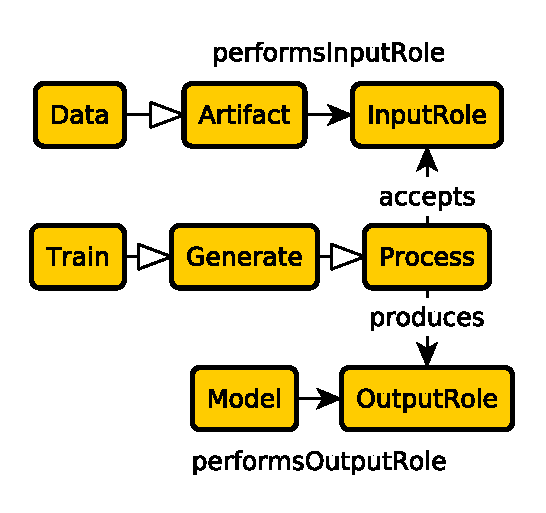
\includegraphics[width=.8\textwidth]{images/schema-diagrams/1a-elementary-pattern.pdf}
\end{center}
\caption{Schema Diagram for the 1a-EASY-AI pattern. %The visual notation is explained in Chapter \ref{chap:prelims}.
}
\label{fig:nen-accepts}
\end{figure}
\subsection{Summary}
Pattern 1a takes an InputRole of artifact-type data which will then participate in a process-type train to produce an OutputRole-type model. 
% 1a describes the interaction between Data as Artifacts being processed through training to produce Models
\label{sum:1a}
%%%%%%%%%%%%%%%%%%%%%%%%%%%%
% Description of 1a-d
%%%%%%%%%%%%%%%%%%%%%%%%%%%%%%%%%%%%%%%%%%%%%%%%%%%%%%%%
\subsection{Axiomatization}
\label{axs:1a}
%%%%%
\textsf{Artifact}-\textsf{performsInputRole}-\textsf{InputRole}
\begin{align}
% General 2, 5, 8, 12, 16
\textsf{Artifact} \sqcap \textsf{InputRole} &\sqsubseteq~\bot \\ %2
% Domain and Range Restrictions
\textsf{$\top$} &\sqsubseteq~\forall\textsf{performsInputRole.InputRole} \\ %5 
% Existential
\textsf{InputRole} &\sqsubseteq~\exists\textsf{performsInputRole}^-\textsf{.Artifact} \\ %8
% Functionality
\textsf{Artifact} &\sqsubseteq~\mathord{\geq}1\textsf{performsInputRole.InputRole} \\ %12
% Inverses
\textsf{InputRole} &\sqsubseteq~\mathord{\geq}1\textsf{performsInputRole}^-\textsf{.Artifact} %16
\end{align}
%%%%%
%%%%%
\textsf{Model}-\textsf{performsOutputRole}-\textsf{OutputRole}
\begin{align}
    % General 2, 5, 8, 12, 16
    \textsf{Model} \sqcap \textsf{OutputRole} &\sqsubseteq~\bot \\ %2
    % Domain and Range Restrictions
    \textsf{$\top$} &\sqsubseteq~\forall\textsf{performsOutputRole.OutputRole} \\ %5 
    % Existential
    \textsf{OutputRole} &\sqsubseteq~\exists\textsf{performsOutputRole}^-\textsf{.Model} \\ %8
    % Functionality
    \textsf{Model} &\sqsubseteq~\mathord{\geq}1\textsf{performsOutputRole.OutputRole} \\ %12
    % Inverses
    \textsf{OutputRole} &\sqsubseteq~\mathord{\geq}1\textsf{performsOutputRole}^-\textsf{.Model} %16
\end{align}
%%%%%
%%%%%
\textsf{Process}-\textsf{accepts}-\textsf{InputRole}
\begin{align}
    % General 2, 3, 4, 5, 7, 12, 16
    \textsf{Process} \sqcap \textsf{InputRole} &\sqsubseteq~\bot \\ %2
    % Domain and Range Restrictions
    \exists\textsf{accepts.$\top$} &\sqsubseteq~\textsf{Process} \\ %3
    \exists\textsf{accepts.InputRole} &\sqsubseteq~\textsf{Process} \\ %4 
    \textsf{$\top$} &\sqsubseteq~\forall\textsf{accepts.InputRole} \\ %5
    % Existential
    \textsf{Process} &\sqsubseteq~\exists\textsf{accepts.InputRole} \\ %7
    % Functionality
    \textsf{Process} &\sqsubseteq~\mathord{\geq}~1\textsf{accepts.InputRole} \\ %12
    % Inverses
    \textsf{InputRole} &\sqsubseteq~\mathord{\geq}1 \textsf{accepts}^-\textsf{.Process} %16
\end{align}
%%%%%
%%%%%
\textsf{Process}-\textsf{produces}-\textsf{OutputRole}
\begin{align}
    % General 2, 3, 4, 5, 7, 12, 16
    \textsf{Process} \sqcap \textsf{OutputRole} &\sqsubseteq~\bot \\ %2
    % Domain and Range Restrictions
    \exists\textsf{produces.$\top$} &\sqsubseteq~\textsf{Process} \\ %3
    \exists\textsf{produces.OutputRole} &\sqsubseteq~\textsf{Process} \\ %4 
    \textsf{$\top$} &\sqsubseteq~\forall\textsf{produces.OutputRole} \\ %5
    % Existential
    \textsf{Process} &\sqsubseteq~\exists\textsf{produces.OutputRole} \\ %7
    % Functionality
    \textsf{Process} &\sqsubseteq~\mathord{\geq}1\textsf{produces.OutputRole} \\ %12
    % Inverses
    \textsf{OutputRole} &\sqsubseteq~\mathord{\geq}1\textsf{produces}^-\textsf{.Process} %16
\end{align}
%%%%%
%%%%%%%%%%%%%%%%%%%%%%%%%%%%%%%%%%%%%%%%%%%%%%%%%%%%%%%%
\subsection{Explanations}
\label{exp:1a}
%%%%%%%%%%%%%%%%%%%%%%%%%%%%
\begin{enumerate}
% Artifact-pIR-IR 2, 5, 8, 12, 16
    \item  Disjointness: \textsf{Artifact} is not \textsf{InputRole}.
    \item  Range: The range of \textsf{performsInputRole} is \textsf{InputRole}. 
    \item   Inverse Existential: For every \textsf{InputRole}, there has to be an inverse R-Filler %for all things that are \textsf{InputRole}, \textsf{performsInputRole} points to it
    \item  Qualified Scoped Functionality: For every \textsf{Artifact}, there is at most one R-filler in \textsf{InputRole} % Every \textsf{InputRole} has at most one \textsf{performsInputRole} that points to it.
    \item  Inverse Qualified Scoped Functionality: for every \textsf{InputRole}, there is at most one inverse R-filler in \textsf{Artifact} % Every \textsf{InputRole}, \txtsf{perfomsInputRole} relates to it. 
% Model-pOR-OR 2, 5, 8, 12, 16
    \item  Disjointness: \textsf{Model} is not \textsf{OutputRole}.
    \item  Range: The range of \textsf{performsOutputRole} is \textsf{OutputRole}. 
    \item   Inverse Existential: For every \textsf{OutputRole}, there has to be an inverse R-Filler %for all things that are \textsf{InputRole}, \textsf{performsInputRole} points to it
    \item  Qualified Scoped Functionality: For every \textsf{Model}, there is at most one R-filler in \textsf{OutputRole} % Every \textsf{InputRole} has at most one \textsf{performsInputRole} that points to it.
    \item  Inverse Qualified Scoped Functionality: for every \textsf{OutputRole}, there is at most one inverse R-filler in \textsf{Model} % Every \textsf{InputRole}, \txtsf{perfomsInputRole} relates to it. 
% Process-accepts-IR 2, 3, 4, 5, 7, 12, 16
    \item Disjoint: \textsf{Process} is not \textsf{InputRole}  %\textsf{Process} are disjoint from \textsf{InputRole}.
    \item Domain: Any value in \textsf{Process} can be assigned to any variable with \textsf{accepts} % Any  \textsf{Process} can be assigned to any \textsf{OutputRole} with \textsf{Accepts}
    \item Scoped Domain: The domain of \textsf{accepts}, scoped by \textsf{InputRole}, is \textsf{Process} % the domain of  \textsf{accepts}, scoped by \textsf{OutputRole}, is \textsf{Process}
    \item Range: the range of \textsf{accepts} is \textsf{Process} % The range of \textsf{accepts} \textsf{OutputRole}
    \item Existential: Every Instance of \textsf{Process} must be related through the relation \textsf{accepts} to some instance within class \textsf{InputRole} %every instance of \textsf{Process} must be related to an \textsf{InputRole} through an \textsf{accepts} relationship
    \item Qualified Scoped Domain: For every \textsf{Process} there is at most one R-filler in \textsf{InputRole} %For every \textsf{Process} there is at most one \textsf{accepts} to \textsf{InputRole}
    \item Inverse Qualified Scoped Functionality: For every \textsf{InputRole} there is at most one inverse R-filler in \textsf{Process} %for every \textsf{InputRole} there is at most one \textsf{accepts} to \textsf{Process}
% Process-produces-OR 2, 3, 4, 5, 7, 12, 16
    \item Disjoint: \textsf{Process} is not \textsf{OutputRole}  %\textsf{Process} are disjoint from \textsf{InputRole}.
    \item Domain: Any value in \textsf{Process} can be assigned to any variable with \textsf{produces} % Any  \textsf{Process} can be assigned to any \textsf{OutputRole} with \textsf{Accepts}
    \item Scoped Domain: The domain of \textsf{produces}, scoped by \textsf{OutputRole}, is \textsf{Process} % the domain of  \textsf{accepts}, scoped by \textsf{OutputRole}, is \textsf{Process}
    \item Range: the range of \textsf{produces} is \textsf{Process} % The range of \textsf{accepts} \textsf{OutputRole}
    \item Existential: Every Instance of \textsf{Process} must be related through the relation \textsf{produces} to some instance within class \textsf{OutputRole} %every instance of \textsf{Process} must be related to an \textsf{InputRole} through an \textsf{accepts} relationship
    \item Qualified Scoped Domain: For every \textsf{Process} there is at most one R-filler in \textsf{OutputRole} %For every \textsf{Process} there is at most one \textsf{accepts} to \textsf{InputRole}
    \item Inverse Qualified Scoped Functionality: For every \textsf{OutputRole} there is at most one inverse R-filler in \textsf{Process} %for every \textsf{InputRole} there is at most one \textsf{accepts} to \textsf{Process}
\end{enumerate}

% %%%%%%%%%%%%%%%%%%%%%%%%%%%%%%%%%%%%%%%%%%%%%%%%%%%%%%%%
% \subsection{Competency Questions}
% \label{cqs:1a}
% %%%%%%%%%%%%%%%%%%%%%%%%%%%%
% \begin{enumerate}[CQ1.]
% \item When was Cogan Shimizu a student at Wright State University?
% \item Who was the lead actor for the movie, Sharknado?
% \item Who was on the World Cup winning team in 2017?
% \end{enumerate}

\newpage
%%%%%%%%%%%%%%%%%%%%%%%%%%%%%%%%%%%%%%%%%%%%%%%%%%%%%%%%
% End Section
%%%%%%%%%%%%%%%%%%%%%%%%%%%%%%%%%%%%%%%%%%%%%%%%%%%%%%%%
%%%%%%%%%%%%%%%%%%%%%%%%%%%%%%%%%%%%%%%%%%%%%%%%%%%%%%%%